\documentclass[12pt,a4paper,twoside]{article}
\usepackage[utf8]{inputenc}
\usepackage{amsmath}
\usepackage{lmodern}
\usepackage{textcomp}
\usepackage{amsfonts}
\usepackage{amssymb}
\usepackage{graphicx}
\usepackage[left=2cm,right=2cm,top=2cm,bottom=2cm]{geometry}
\author{Cabello Lopez Marco Antonio\\
Actividad 4 \\
Departamento de Fisica\\
Universidad de Sonora}
\date{Hermosillo, Sonora a Viernes 27 de Octubre del 2017}
% used in maketitle                                                             
\title{\textbf{Movimiento de un Proyectil con Resistencia al Aire}}
\begin{document}
\maketitle
\section{Planteamiento del problema}
En esta actividad se pide primeramente, desarrollar las ecuaciones de movimiento para un proyectil que se mueve en la atmósfera y que sufre resistencia del aire. Una vez completado esto, pasaremos a resolver numéricamente el problema, apoyados con Fortran.

Apoyandonos con las notas de movimiento de Richard Fitzpatrick de la Universidad de Texas y el metodo de euler para la integracion.

\begin{figure}[h!]
  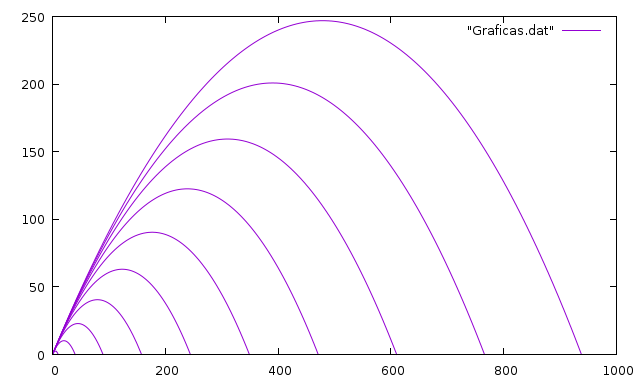
\includegraphics[width=\linewidth]{sistema.png}
  \caption{Grafica de posiciones}
  \label{fig:Grafica}
\end{figure}

\begin{verbatim}
program movimientoproyectil
  implicit none
  !Definimos las variables reales
   real :: vt, c, area, vter, fi, fj, t, a
  !Definimos las variables reales con parametros
   real, parameter :: deltat = .01, m = 0.250, r = 0.05, cd = 0.47
   real, parameter :: u = 2 , g = 9.81, pi = 3.1415927, Ro = 1.225
  !Definimos las variables 
   real, dimension(100000) :: x, y, vx, vy
  !Definimos las variables enteras
   integer :: i, j
   integer, parameter :: maxvel = 100, ntimes = 100000
   
!Calculamos el Area del circulo.
   area = pi * r * r
!Calculamos la velocidad terminal.
  vt = ((2 * m * g) / (Ro * area * cd))
  vter = SQRT(vt)
!Calculamos el coeficiente de fricción.
 c = (m * g) / (vt)
!Calculamos el angulo en radianes
a = 45 * pi / 180.0

   open(1, file='Graficas.dat', status='unknown')

 do j=10, maxvel, 10
    fj = float(j)
    
     do i=1, ntimes
       fi = float(i)
       t = fi * deltat
       
     if (i.LT.3) then
     
     vx(i) = fj * cos(a)
     vy(i) = fj * sin(a) - (g * t)

     x(i) = fj * t * cos(a)
     y(i) = fj * t * sin(a) - 0.5 * g * t * t

     end if

     if (i.GT.2) then
     vx(i) = vx(i-1) * (1 - deltat * c / m)
     x(i) = x(i-1) + deltat * vx(i-2) * (1 - deltat * c / m)

     vy(i) = vy(i-1) * (1-deltat * c / m) - deltat * g
     y(i) = y(i-1) + deltat * vy(i-2) - deltat * deltat * g + deltat * c / m * vy(i-2)
     

     if (y(i).LT.0) exit
     
     end if
     
       write(1,*) x(i), y(i)
       
    
     end do
       write(1,*) ' '
 end do
     
    close(1)
    
 

  end program movimientoproyectil
\end{verbatim}




\end{document}
